\documentclass{article}
\usepackage{graphicx}
\usepackage[margin=2cm]{geometry}
\usepackage{hyperref}
\usepackage{cite}
\usepackage{subcaption}

\title{\Huge \textbf{AppleStocks}\\\vspace{0.2em} \Large A Simple Application for Apple Stock Quotes Monitoring}
\author{
    Henrique Romão \\ 
    \textit{up202108067@up.pt} 
    \and 
    Mariana Bessa \\ 
    \textit{up202107946@up.pt}
}

\setlength{\parindent}{0em}
\setlength{\parskip}{0.7em}
\setcounter{tocdepth}{2}
\begin{document}

\maketitle

\hfill

\tableofcontents

\hfill

\newpage

\section{Introduction}
In this small project we develop a simple and effective mobile device application to display closing stock prices of Apple Inc.
The information is displayed according to two factors choosen by the user: time period type — hours or days —; and the number of time periods to showcase — from 2 to 10.
The application is divided into two activities, one responsible for getting the user choices, and another responsible for processing the data retrieved from the internet and plotting the processed data.
The design is simple, ensuring the application is ease to use, in hopes of increasing acessability and, therefore, the potential number of users.

\section{Use Cases}
The application supports the following use cases, which are represented in the use case diagram, in \autoref{fig:UseCases}.

\paragraph{Choose View Options}
Where the user selects a time interval, Hourly or Daily, and a range, 2–10.
\vspace{-0.5em}

\paragraph{Get Stock Information}
Where the application connects with the Web API.
\vspace{-0.5em}

\paragraph{See Stocks}
When the user pushes the "Submit" button and sees the Plot Activity.
\vspace{-0.5em}

\begin{figure}[ht]
    \centering
    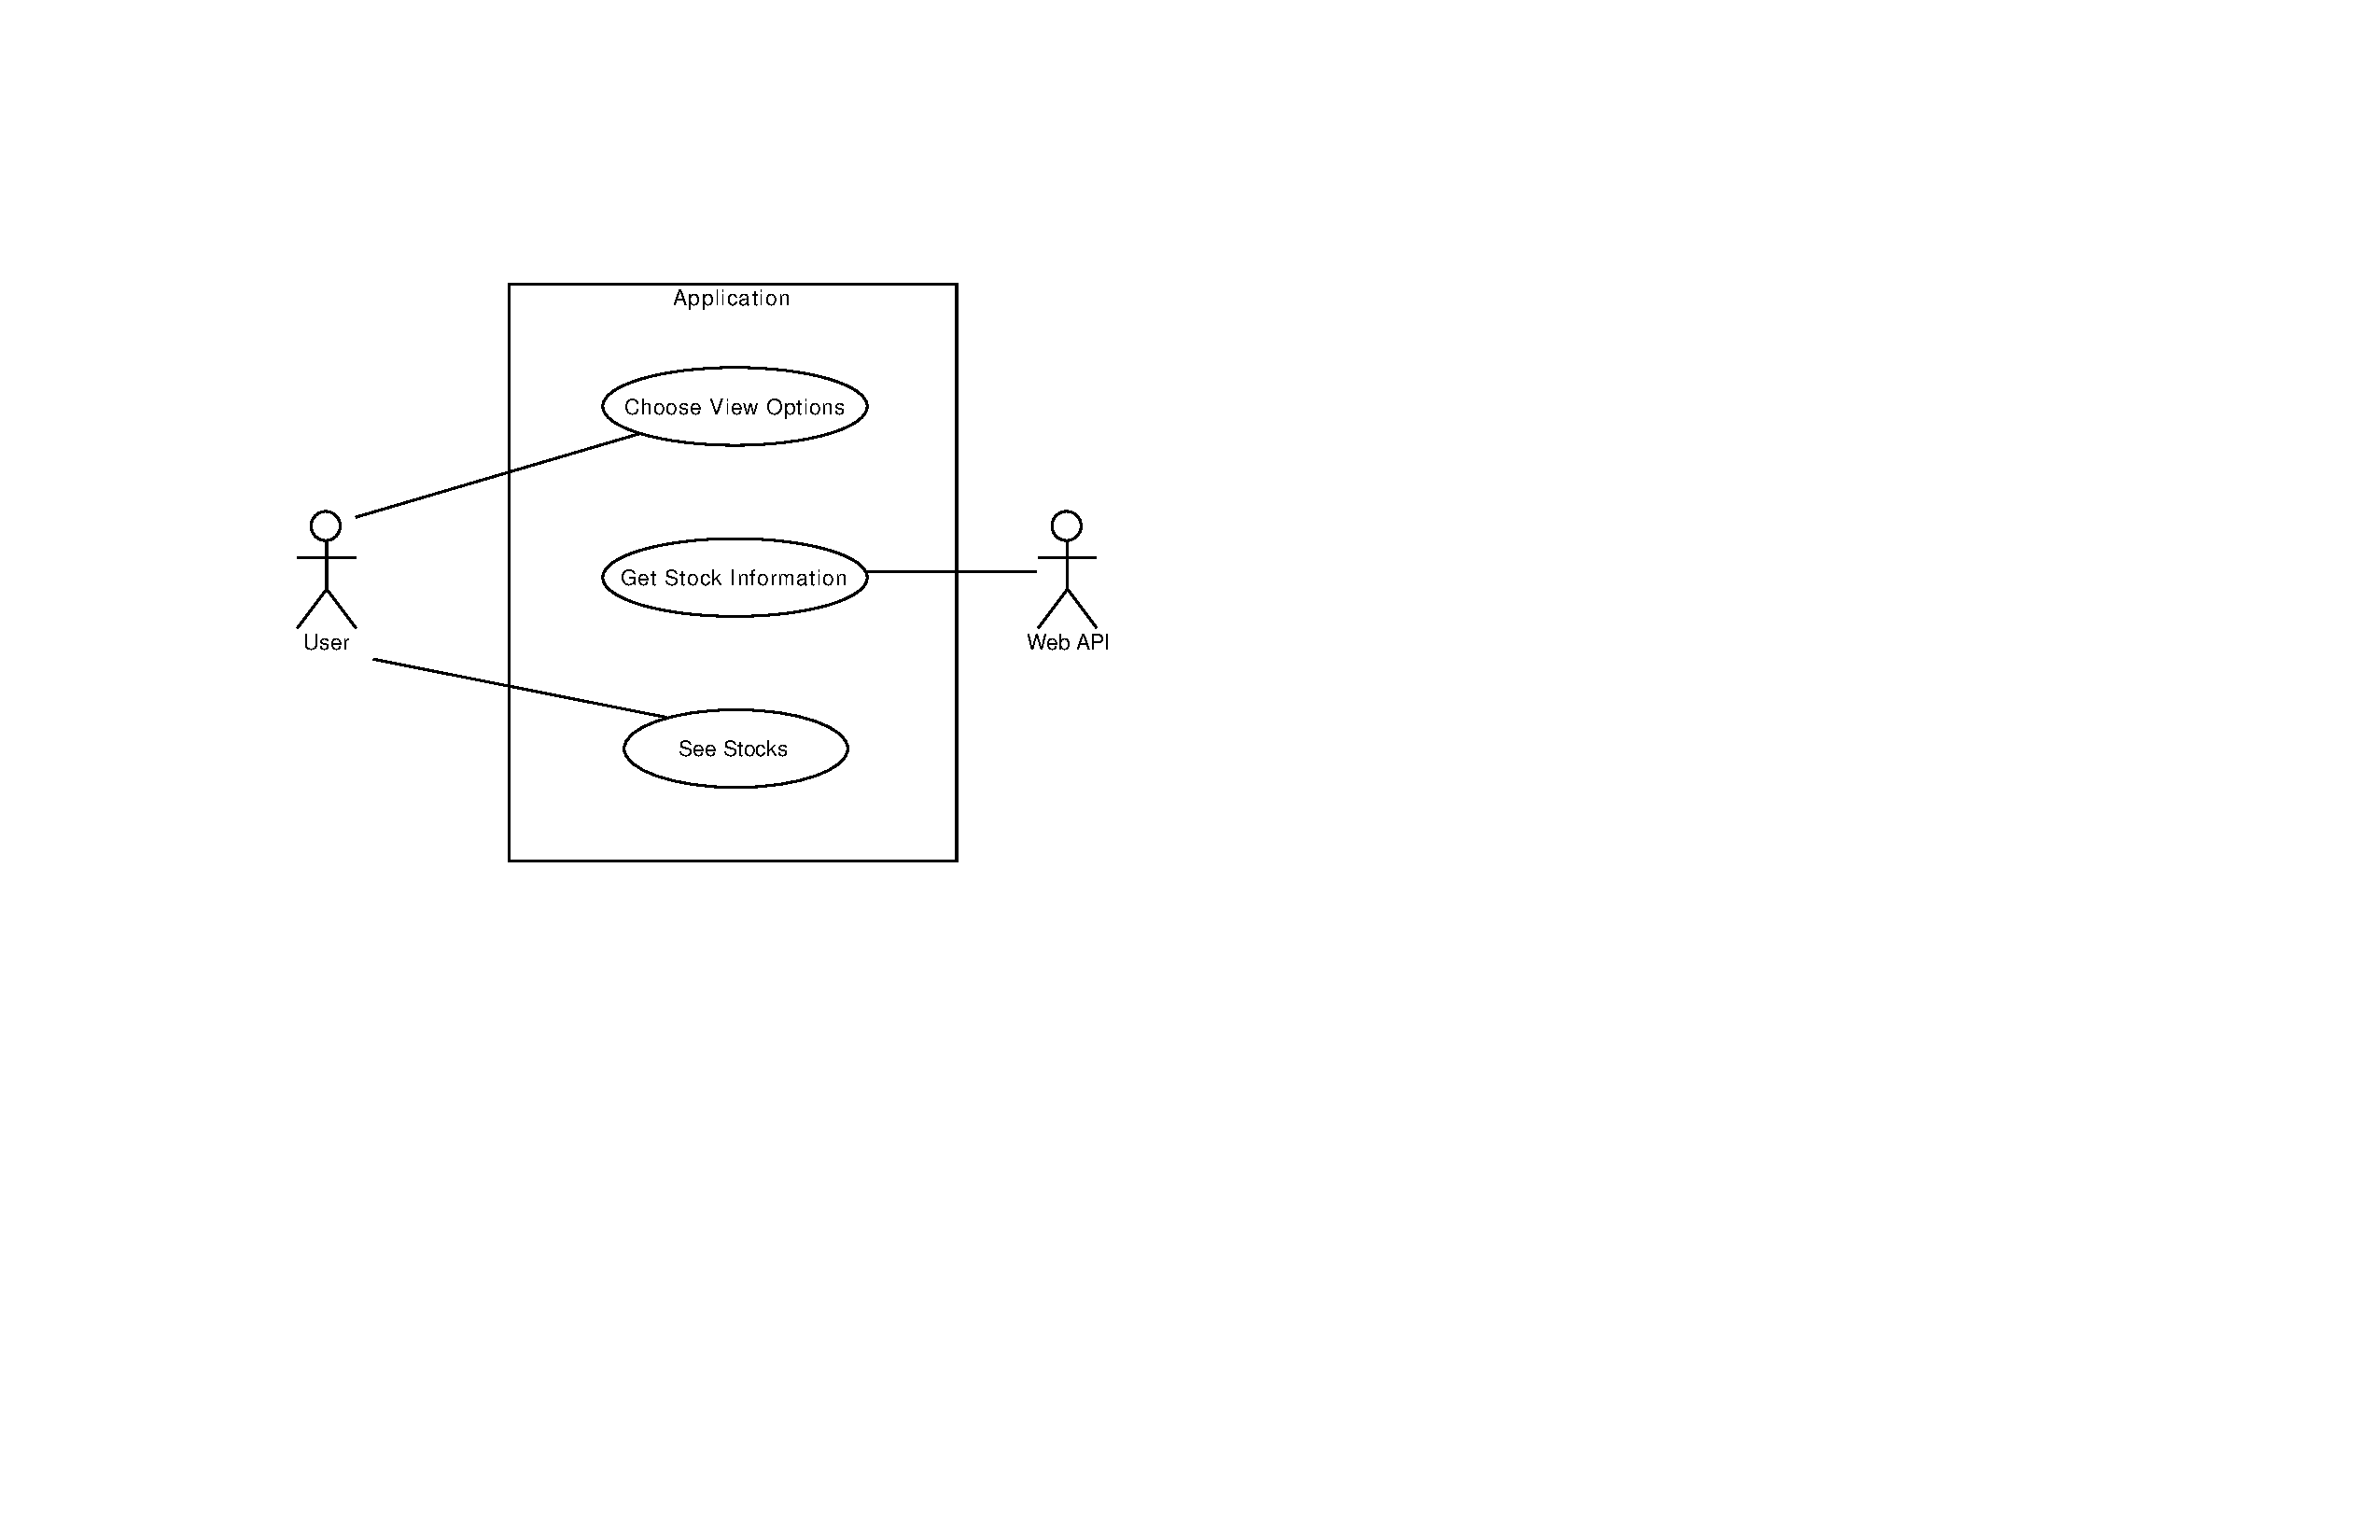
\includegraphics[width=0.6\linewidth]{Use Cases.pdf}
    \caption{Use Cases Diagram.}
    \label{fig:UseCases}
\end{figure}



\section{Architecture}
To make the application more user-friendly and the interface less crowded, the application was divided into two activities: the Main Activity, where the user configures their preferences, and the Plot Activity, where the results are displayed.
Common to both activities, there is an action bar displaying the name of the app. 

\subsection{Main Activity}
\label{sec:Main Activity Java}
This activity also includes two \texttt{Spinner} objects: one for selecting the type of interval (hours or days) and another for specifying the interval range. 
These spinners are initialized in the Main Activity code using the \texttt{new ArrayAdapter<>()} method, with \texttt{setDropDownViewResource()} used to define their layout.

Both spinners have default values: ``H" (hours) for the type of interval and ``2" for the range. 
This means that, unless changed by the user, the stock quotes for the last two hours will be displayed by default.

A button is provided to allow the user to proceed, with its listener being implemented within the Main Activity. The \texttt{onClick()} method creates an \texttt{Intent} to open the Plot Activity, passing the user's spinner selections (as a string and an integer) to the new activity.


\subsection{Plot Activity}
The plot activity is where, according to the choices made on the Main Activity, the HTTP request is made, retrieving the stock information from the web API, and it is also in this activity that the retrieved information is processed and displayed to the user.

\subsubsection{HTTP Request}
The first step to retrieve the information from the web API is to read the intent passed from the previous activity, with the time interval type and number.
With these two variables, it is possible to craft the URL, which will be used to do the HTTP request.
This URL is passed through a function that initiates a new thread, where the rest of the processing will take place.
Inside the thread, the processing will be initiated by \texttt{FetchData}, a private class that takes a URL and establishes the HTTP connection.
The connection status is then assessed, and if it is succesfull, the processing will go on; otherwise, an error message is thrown.

\subsubsection{Data Processing}
Before the actual processing begins, the input stream received from the HTTP connection is converted into type \texttt{String}.
With this \texttt{String}, function \texttt{processJsonData} will create a JSON object to retrieve the closing quote prices and respective time.
Redarding the time, it is necessary to convert the dates into float type objects, for the plot function, and so it is necessary to format the dates.

A problem that arises is that, according to the choice of days or hours, the date format will be different, as, in the las case, it will include the hour and timezone.
According to the selected time interval type passed through the intent, a different format will be used for parsing the date strings into date objects, which are then converted to floats with the timestamps.
The processed information is then passed to the \texttt{plotData} function.

\subsubsection{Data Plotting}
The data is plotted using the LineData widget, part of the MPandroid Chart library, \cite{MPAndroidChart}.
A widget was used to take advantage of already developed code and shorten the app development period.
This particular widget was choosen due to its widespread use, seeming a correct fit for the task in hand.

In this widget the data is passed in an array of entries, and so the function joins the two arrays into a single array of entries with two values, one entry for each dot in the plot.
Additionally, the function computes the maximum and minimum closing quote prices, and creates an entry array for each, to be plotted as horizontal lines delimiting those values.
Then, each entry array is properly formatted, and sent to the widget to be plotted.
It is also necessary to format the x-axis, otherwise the values seen would be the float type objects, which are difficult to interpret and not user-friendly.
To this intent, the value is formatted to return a simple date string, and only the first and last values are shown, for a simpler graph analysis.
The maximum and minimum values are also shown outside the plot.

\section{Interface}
The application has a black background with purple accents, as darker colors are more associated with the stock tracking and the stock market. The theme used was \texttt{Theme.AppCompat.Light.DarkActionBar}.

The interface is structured using \texttt{LinearLayout} objects to arrange the \texttt{TextView} elements, \texttt{Spinner} objects, and \texttt{Submit} button in vertical and horizontal sequences. When the \texttt{Submit} button is pressed, the application starts the \texttt{Plot Activity} using the \texttt{startActivity()} method, passing the selected user inputs as extras, in the intent.

\subsection{Main Activity}
This activity is design to adapt to both horizontal (landscape) and vertical (portrait) screen orientations, maintaining a consistent and user-friendly layout.

\subsubsection{Portrait}
Upon opening the application, the user is welcomed by an action bar and two \texttt{TextView} elements, where one displays a greeting, and the other provides instructions on how to use the application, as it is shown in \autoref{fig:mainactivity}. 
Below these, additional \texttt{TextView} elements explain the purpose of each \texttt{Spinner} object, which are used for input selection.

The layout for the spinner items and their drop-down lists was custom-designed in the XML files \texttt{/layout/spinner \_dropdown\_item.xml}, which defines the appearance of the spinner drop-down items, and \texttt{/layout/spinner\_item.xml}, which defines the appearance of the selected spinner items (\autoref{fig:spinner1} and \autoref{fig:spinner2}).
It should be noticed that the spinner items are scrollable.
The spinner values are defined in the \texttt{strings.xml} file located in \texttt{/res/values/}. 


Additionally, custom shapes were created to style the \texttt{Submit} button and the background of the spinner section. 
These shapes were implemented in the \texttt{/drawable/submit\_button.xml} file, which defines the shape of the Submit button, and the \texttt{/drawable/round\_button.xml} file, which shapes the background of the selection area.


\begin{figure}[ht]
    \centering
    
    \begin{subfigure}[t]{0.30\linewidth}
        \centering
        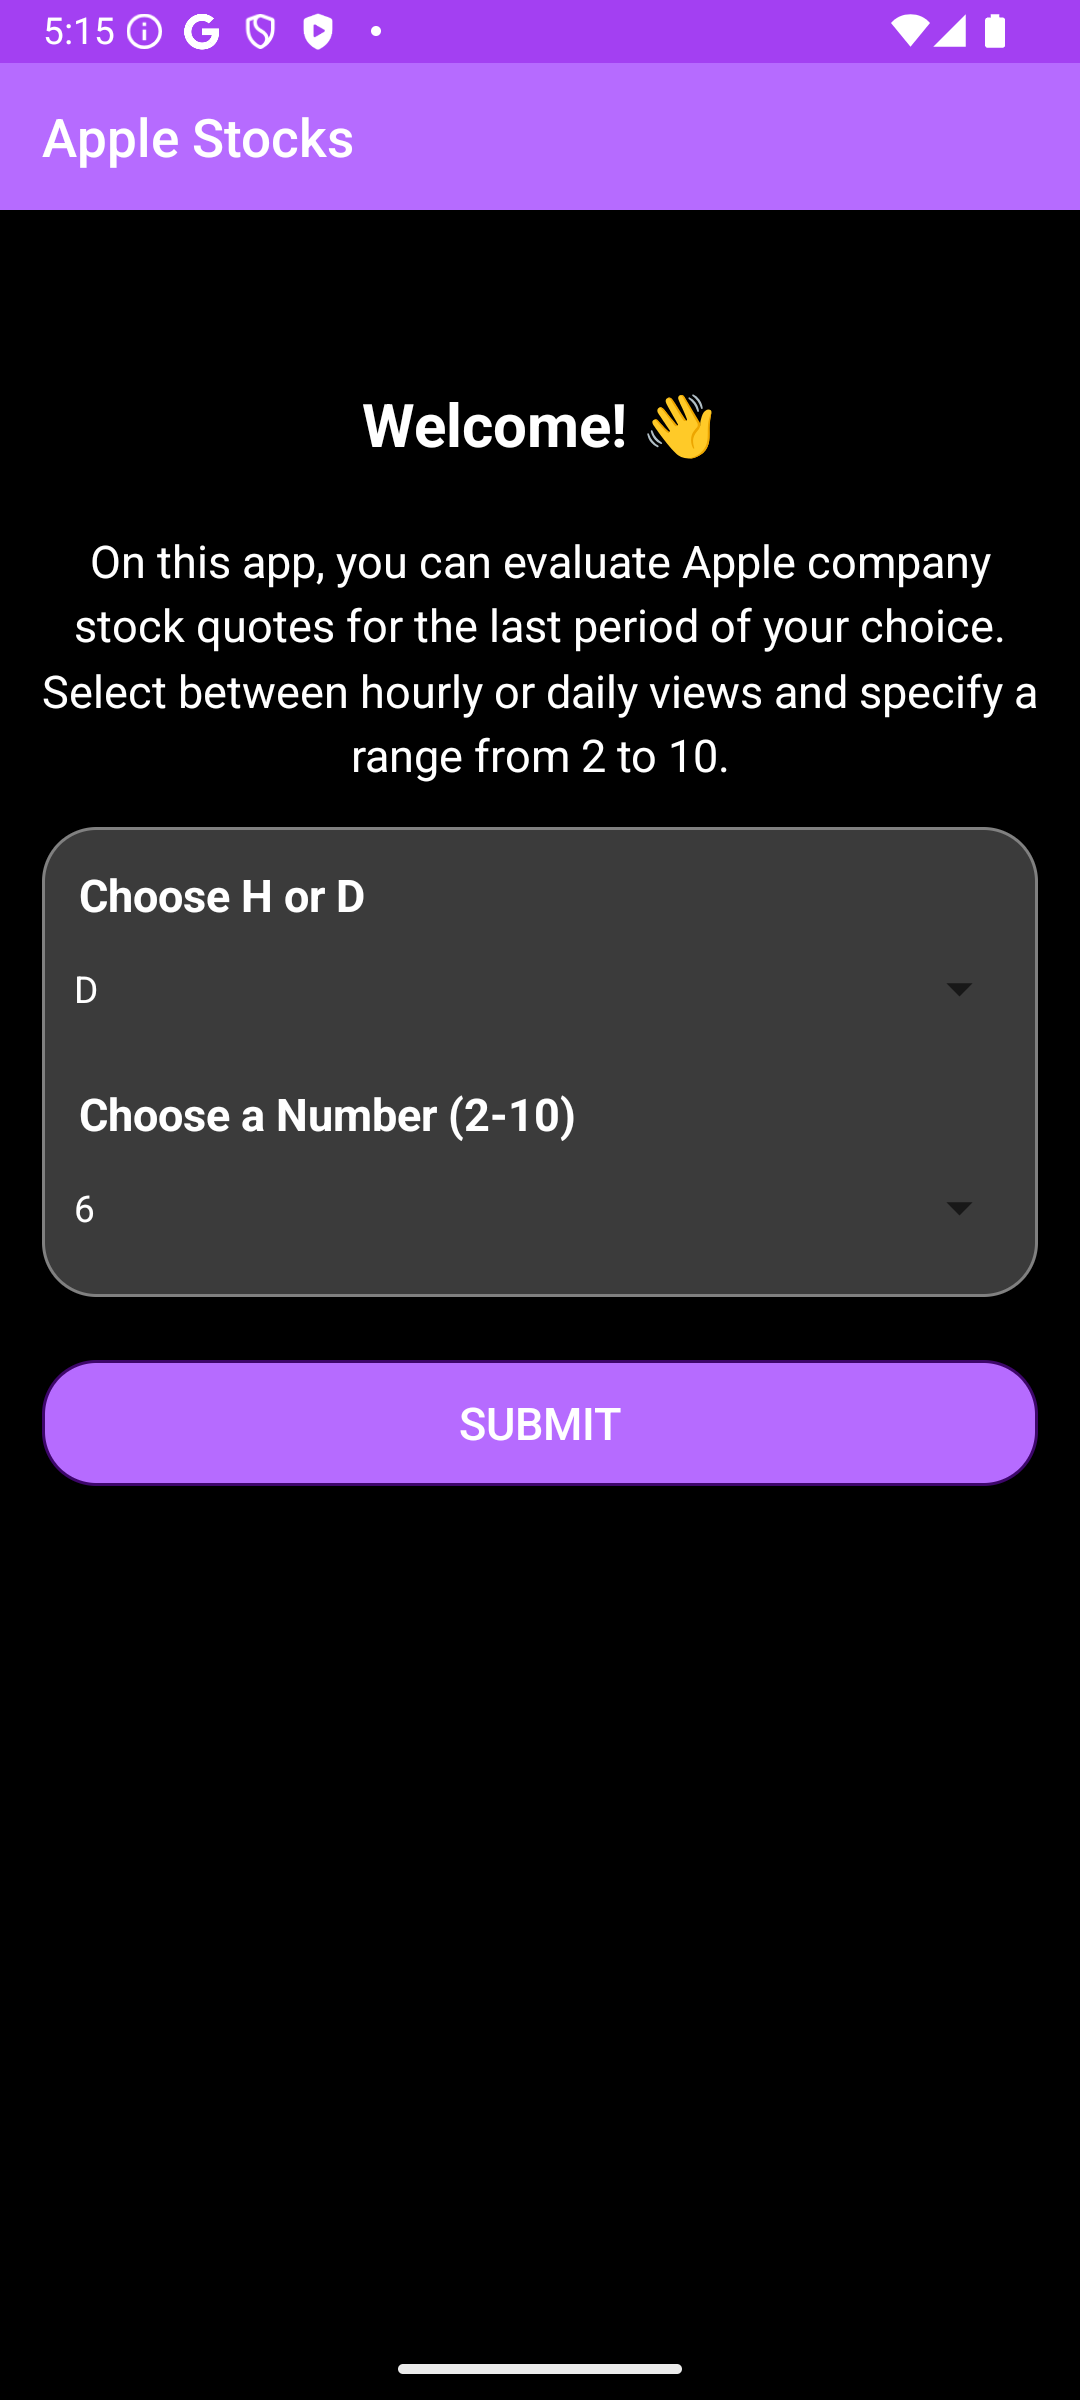
\includegraphics[height=30em]{Imagens/Main Activity.png}
        \caption{Main Activity.}
        \label{fig:mainactivity}
    \end{subfigure}
    \hfill
    \begin{subfigure}[t]{0.30\textwidth}
        \centering
        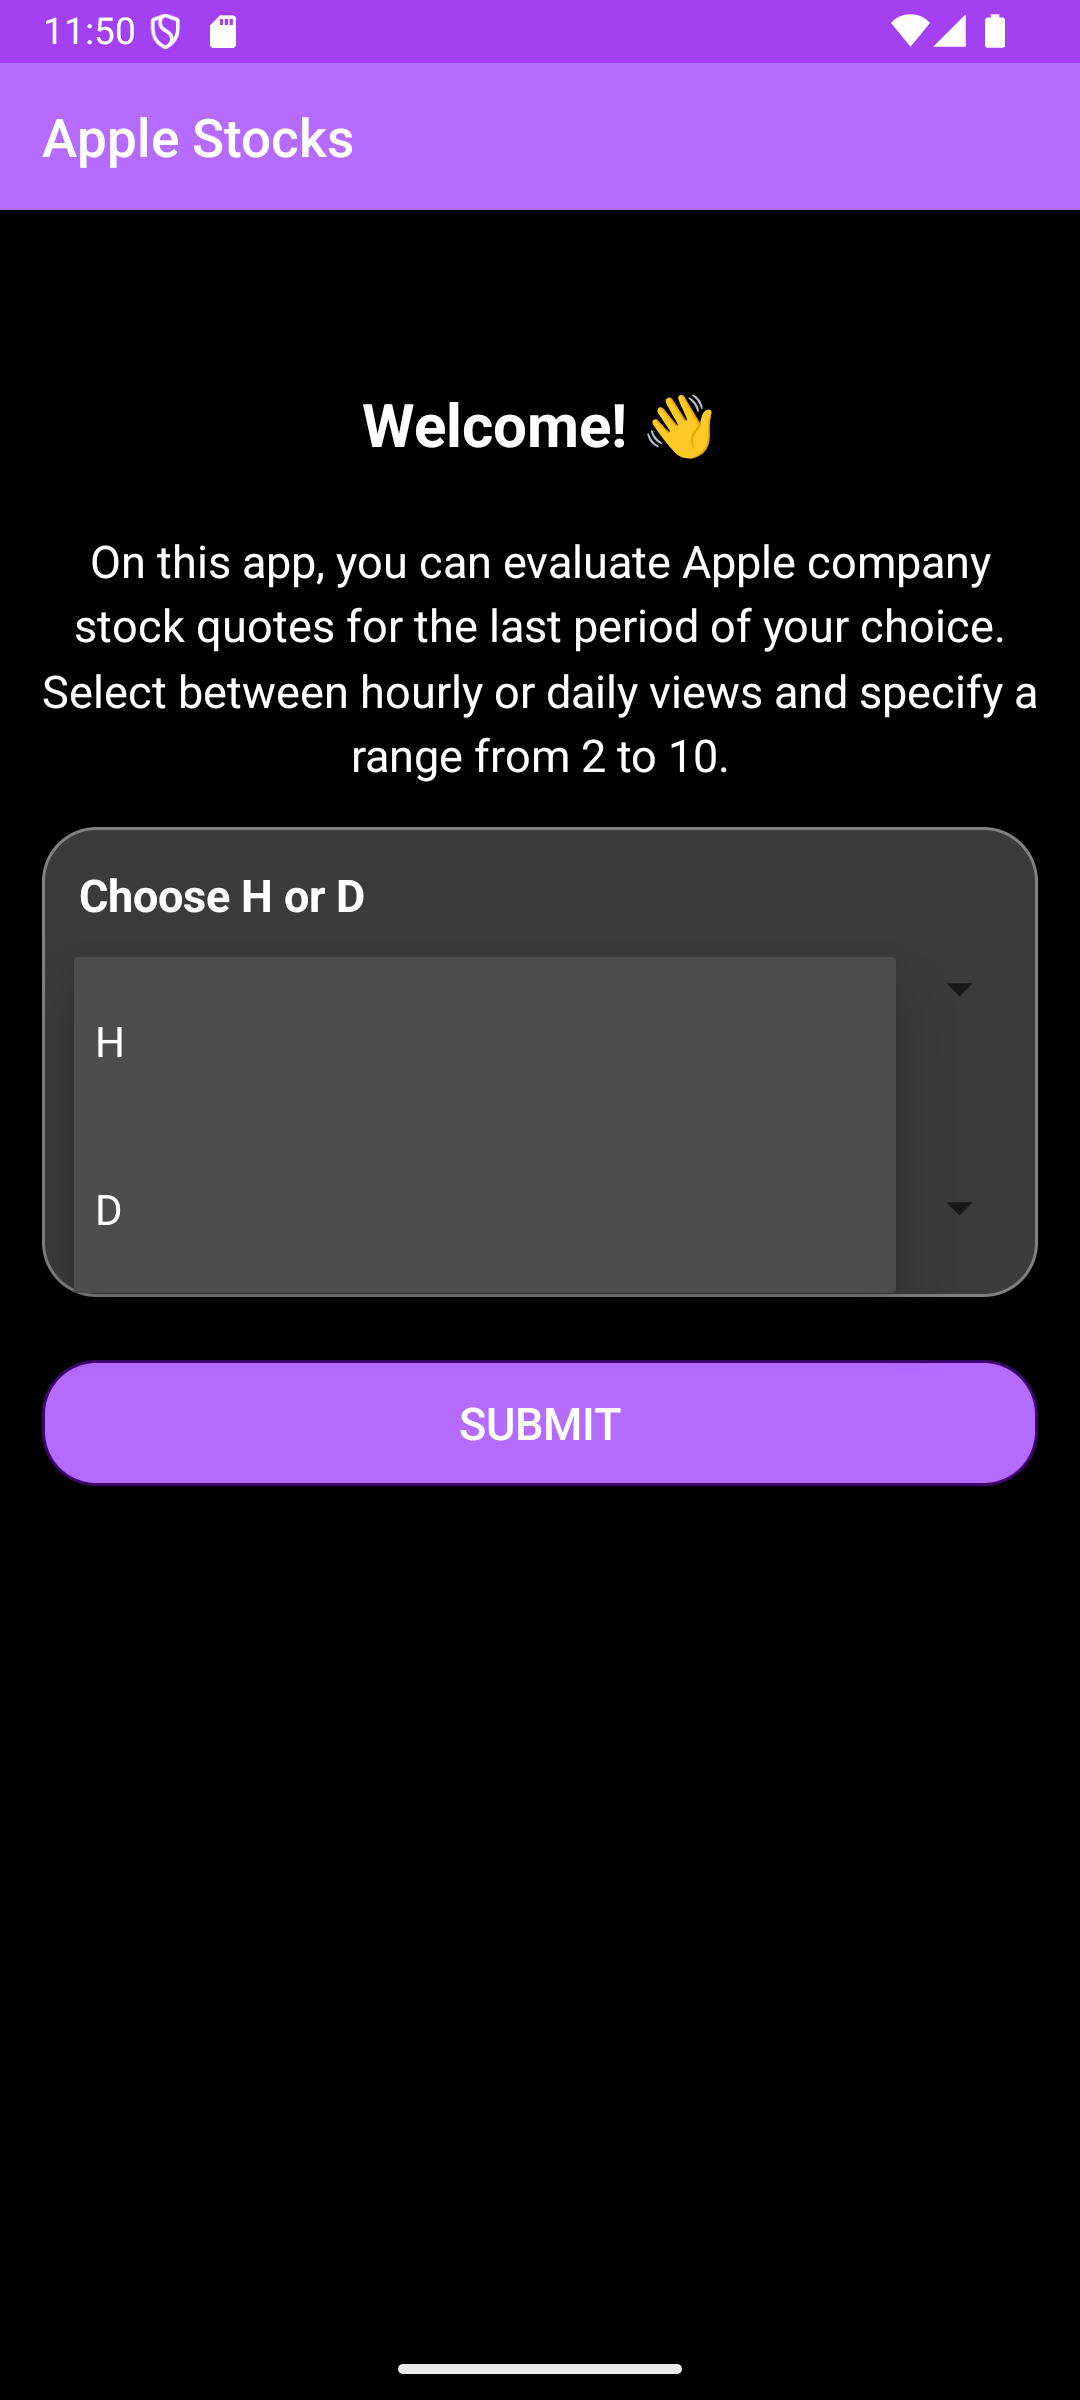
\includegraphics[height=30em]{Imagens/Spinner1.png}
        \caption{Interval Choice.}
        \label{fig:spinner1}
    \end{subfigure}
    \hfill
    \begin{subfigure}[t]{0.30\textwidth}
        \centering
        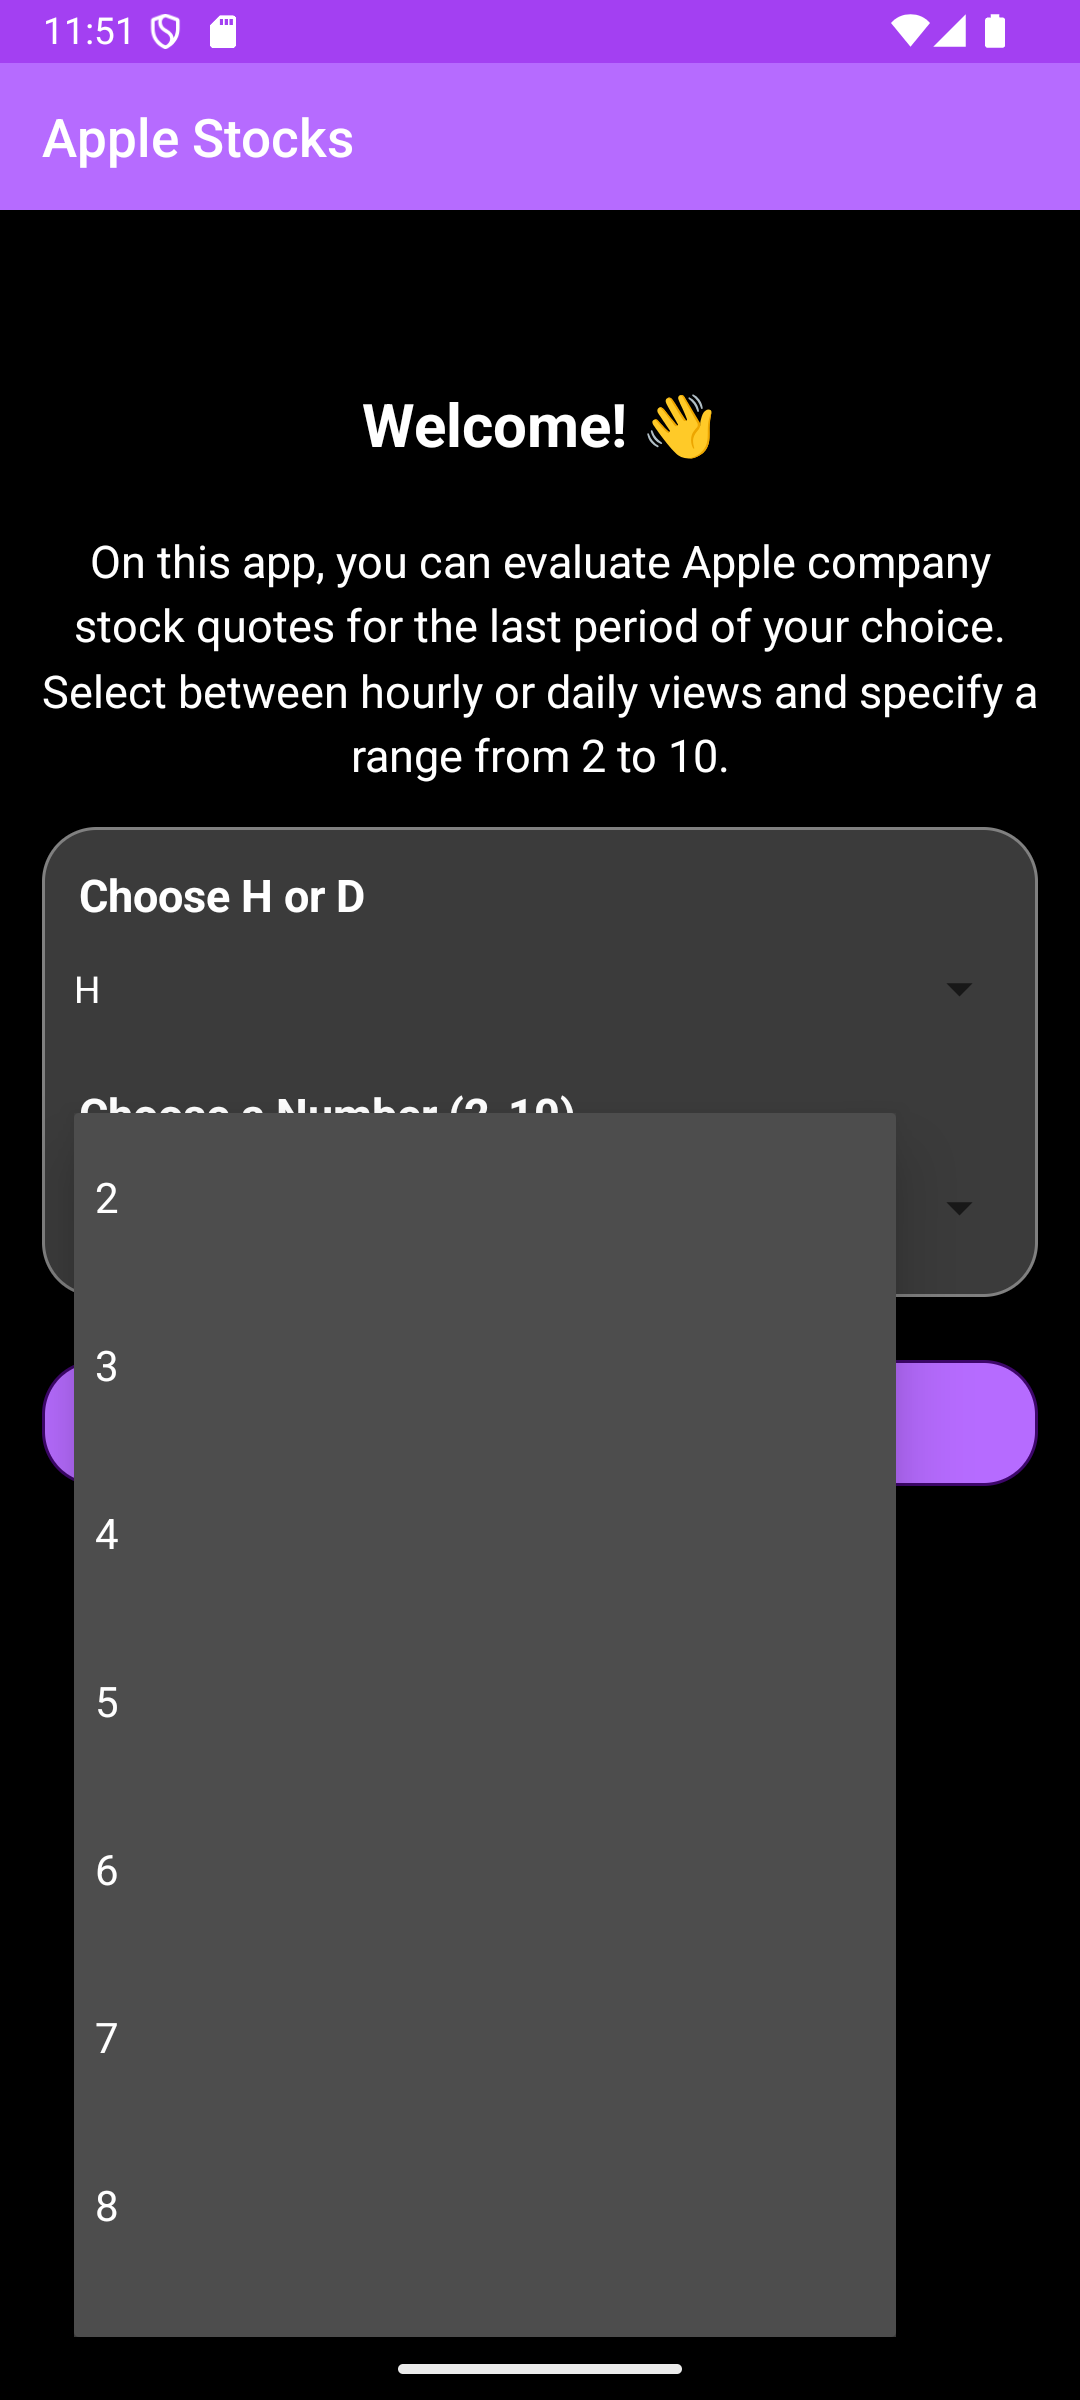
\includegraphics[height=30em]{Imagens/Spinner2.png}
        \caption{Range Choice.}
        \label{fig:spinner2}
    \end{subfigure}

    \caption{Main Activity.}
    \label{fig:whole main activity}
\end{figure}

\subsubsection{Landscape}

In the landscape orientation, a dedicated layout file, \texttt{/layout-land}, was created to optimize the user interface for horizontal screens. 

This layout maintains the key aspects of the portrait view, with the main adjustment being the rearrangement of the \texttt{Spinner} objects: instead of being vertically aligned, they are displayed side by side (horizontally). This design enhances usability by taking full advantage of the horizontal screen space.

The layout is shown in \autoref{fig:mainactivity_l}, including the spinner options for interval and range choices (\autoref{fig:spinner1_l} and \autoref{fig:spinner2_l}).

\begin{figure}[ht]
    \centering
    \begin{subfigure}[t]{0.8\textwidth} 
        \centering
        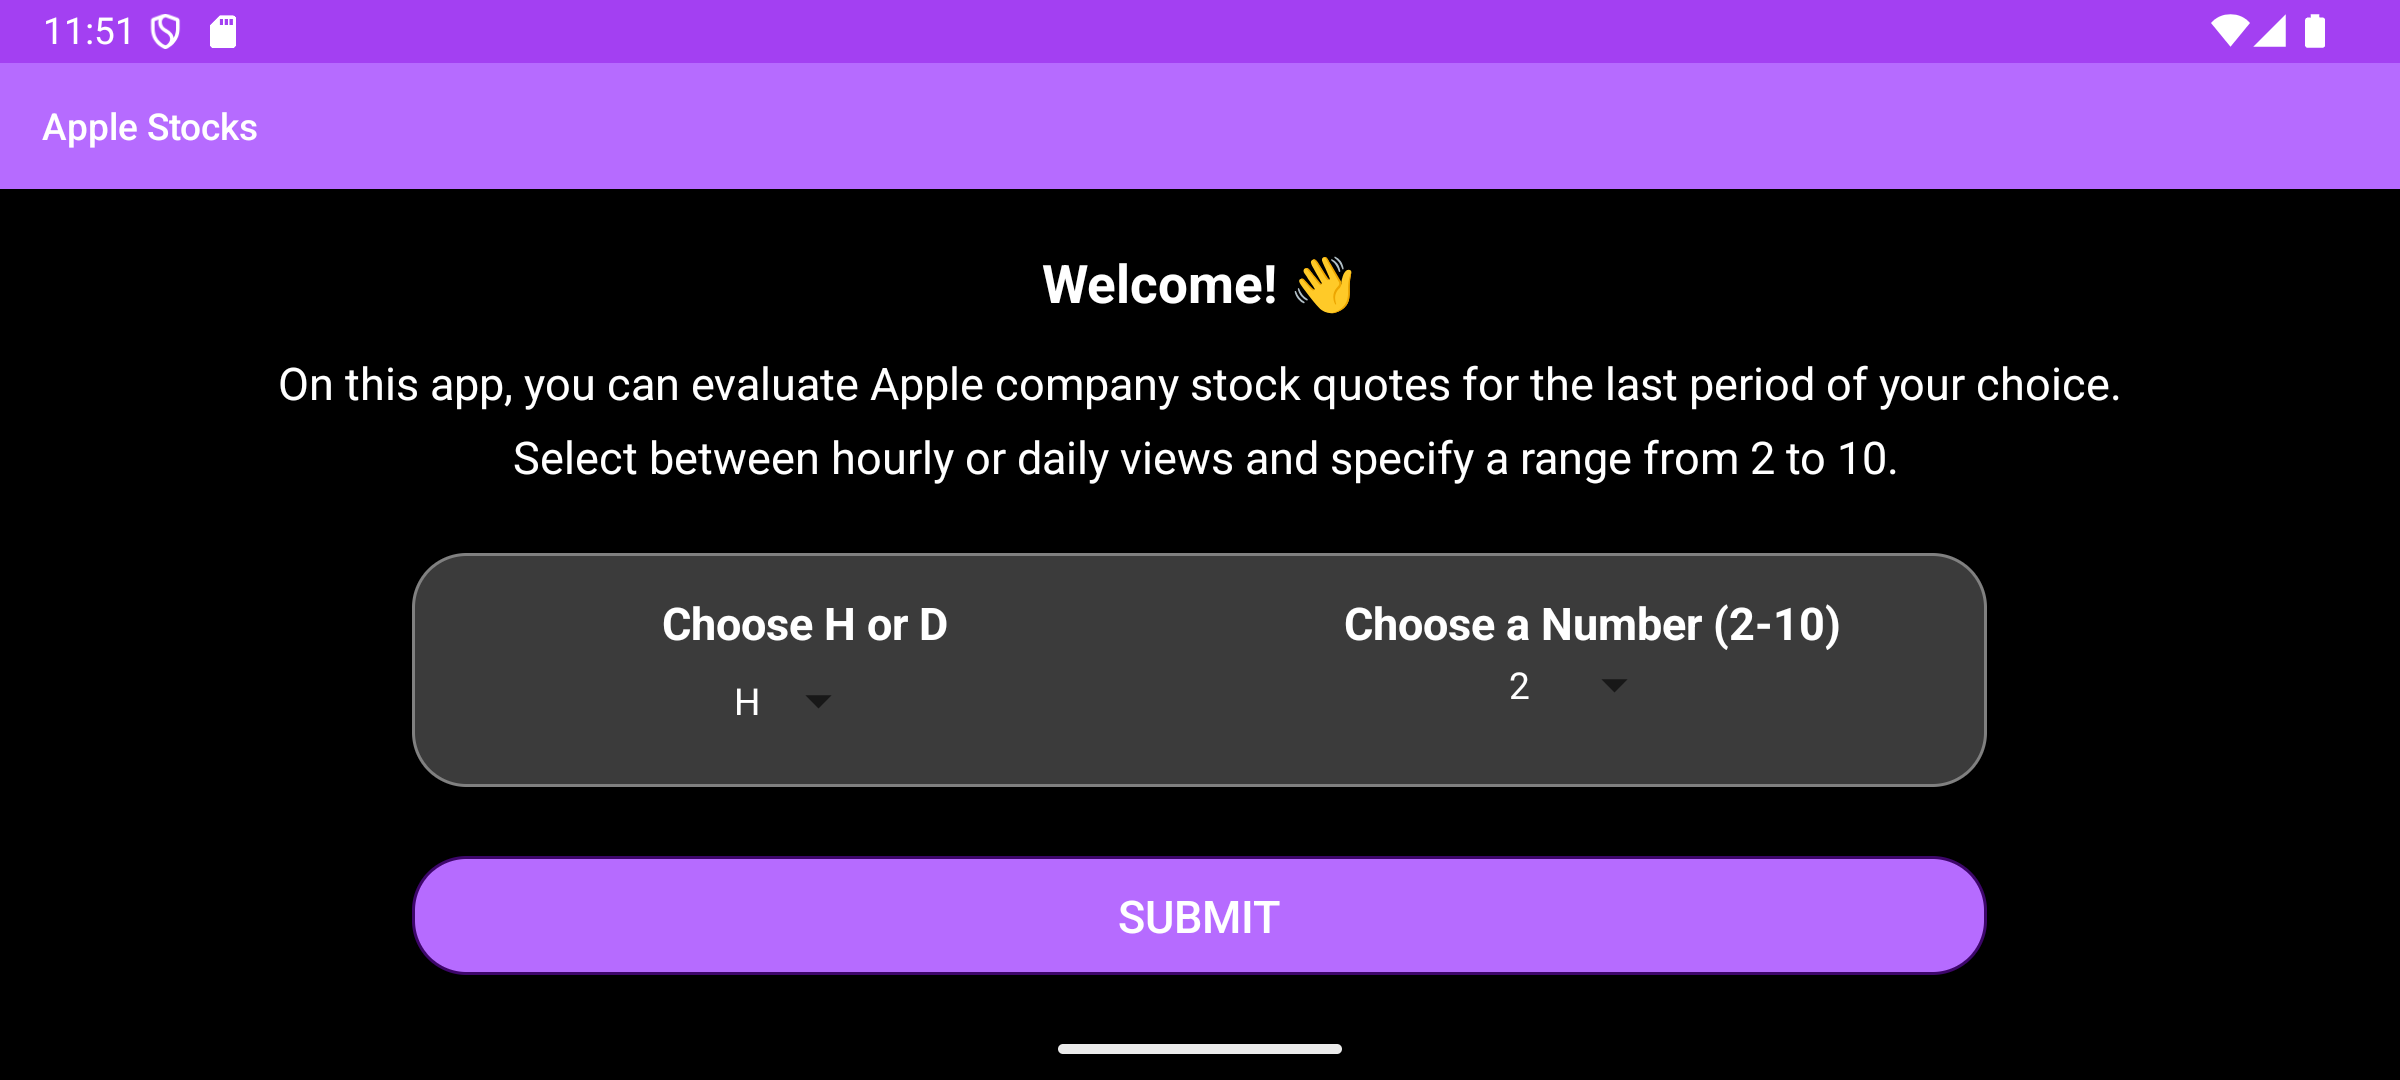
\includegraphics[width=\textwidth]{Imagens/Main_Landscape.png}
        \caption{Main Activity.}
        \label{fig:mainactivity_l}
    \end{subfigure}

    \vspace{1em} 

    \begin{subfigure}[t]{0.8\textwidth}
        \centering
        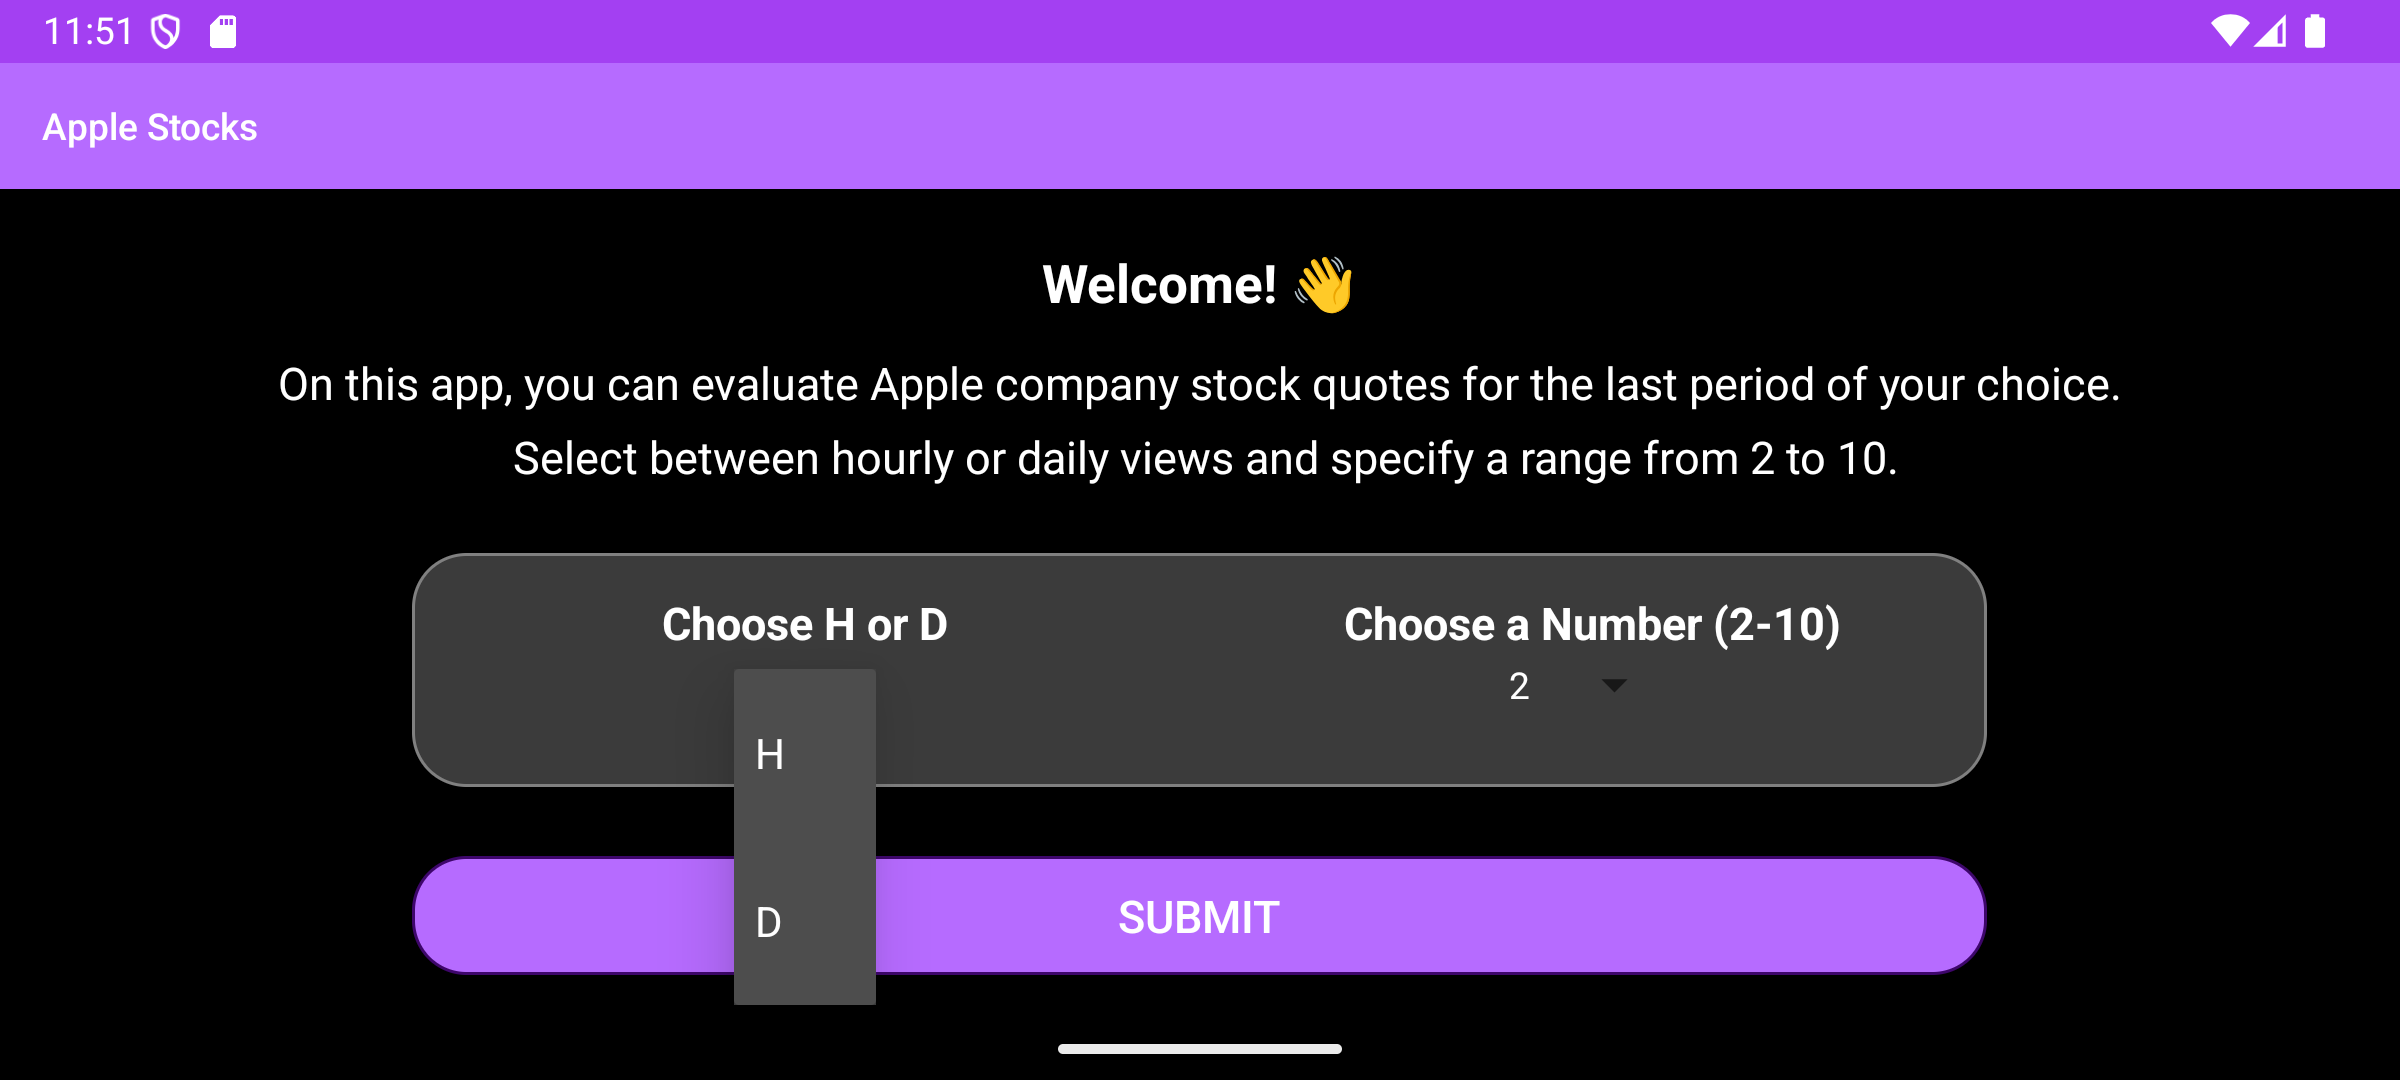
\includegraphics[width=\textwidth]{Imagens/Spinner1_landscape.png}
        \caption{Interval Choice.}
        \label{fig:spinner1_l}
    \end{subfigure}

    \vspace{1em} 

    \begin{subfigure}[t]{0.8\textwidth}
        \centering
        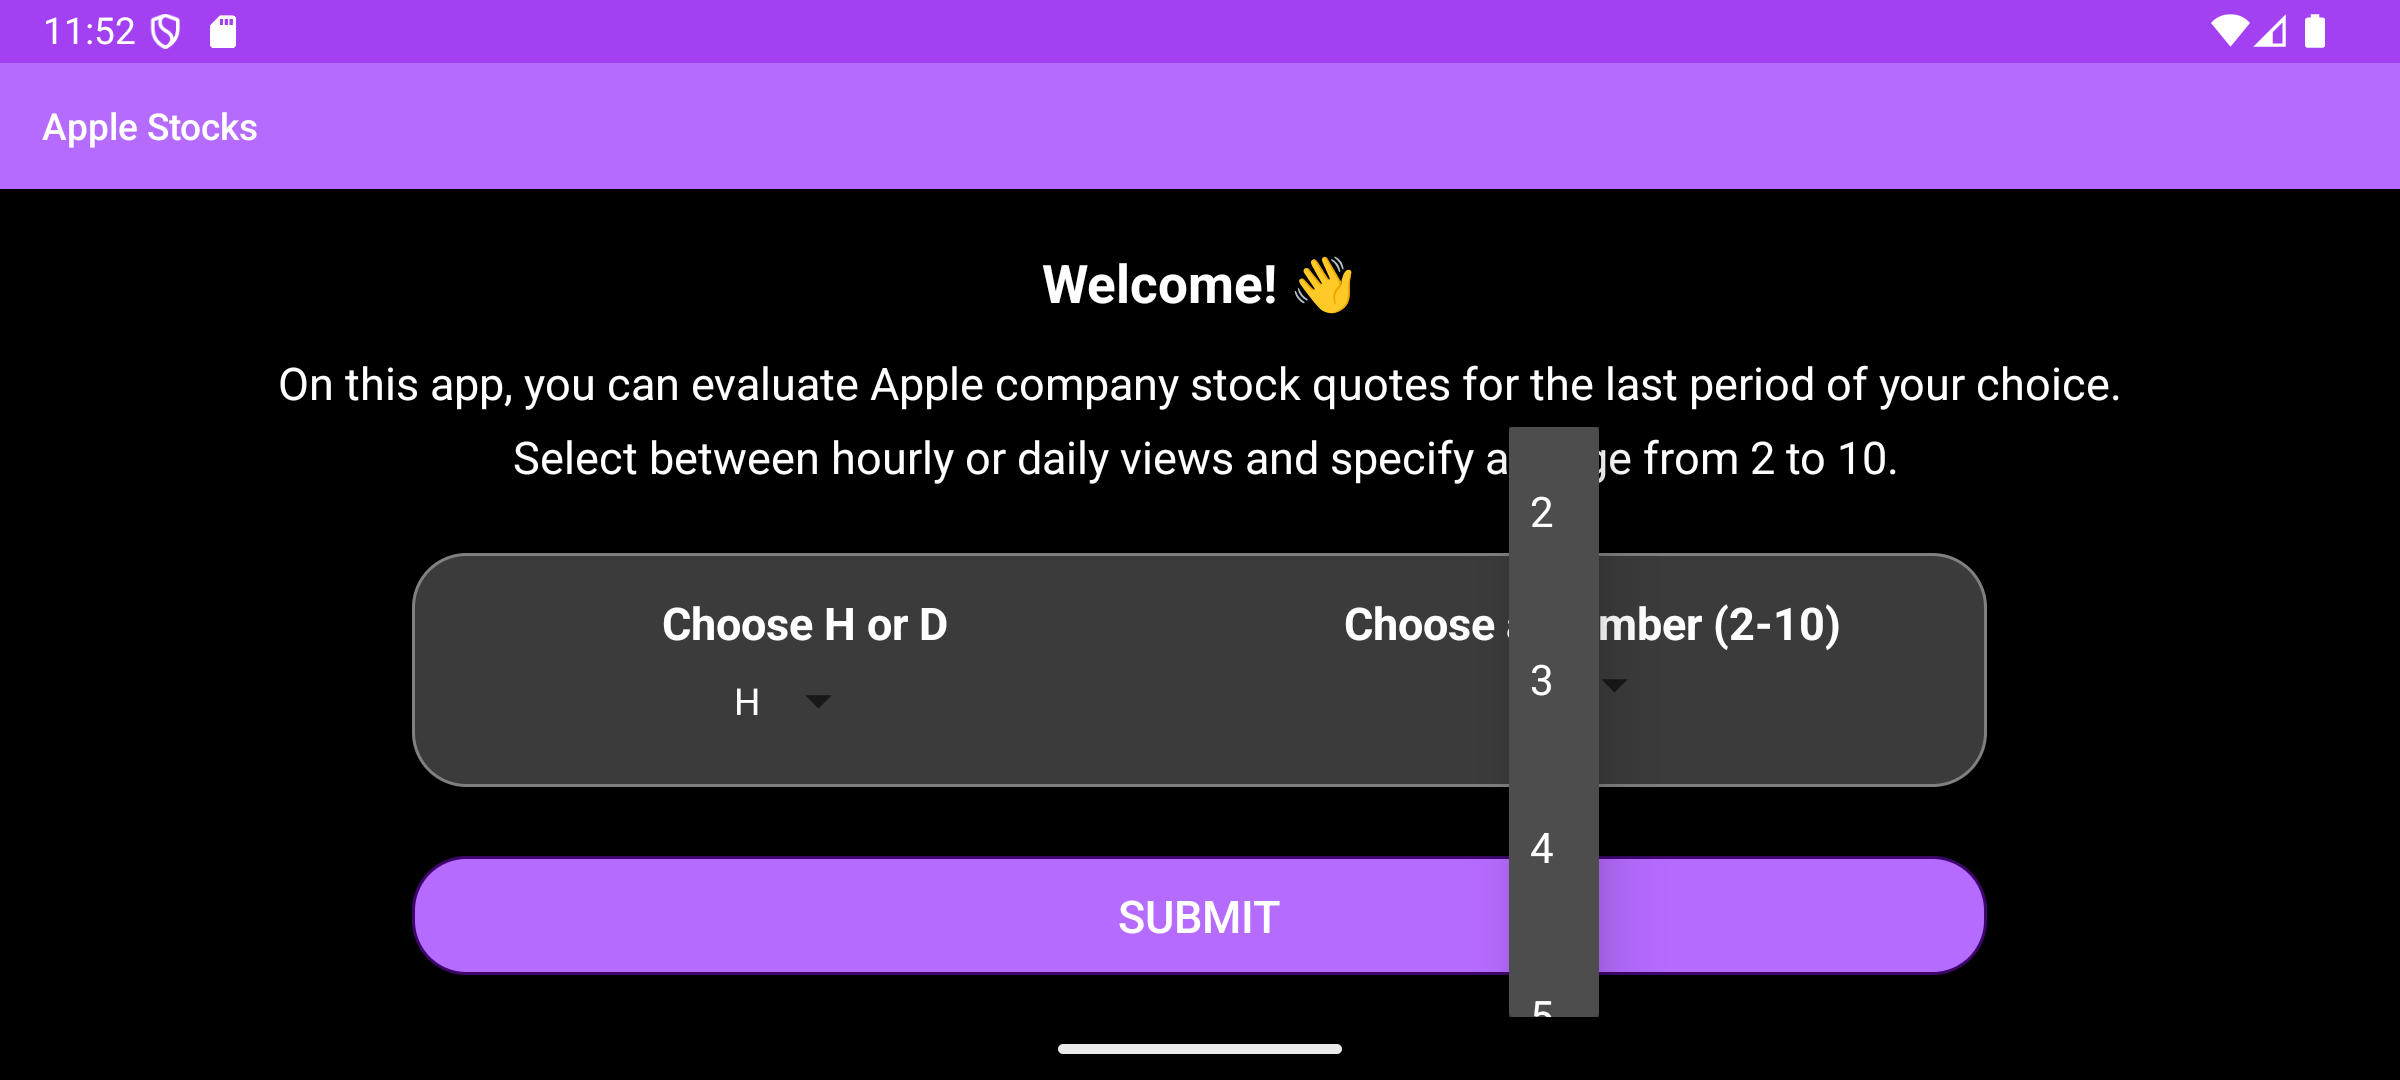
\includegraphics[width=\textwidth]{Imagens/Spinner2_landscape.png}
        \caption{Range Choice.}
        \label{fig:spinner2_l}
    \end{subfigure}

    \caption{Main Activity in Landscape.}
    \label{fig:whole_main_activity}
\end{figure}

\subsection{Plot Activity}
The interface for the plot activity can be seen in \autoref{fig:plot activity}, with the activity still loading the data (\autoref{fig:loading}) and with all the data loaded (\autoref{fig:plot loaded}).
The activity takes some time loading, but this wait is due to slow connectivity of the web API, having tested the speed for the same request in our personal computers and noticing a slight delay.

\begin{figure}[ht]
    \centering
    
    \begin{subfigure}[t]{0.49\textwidth}
        \centering
        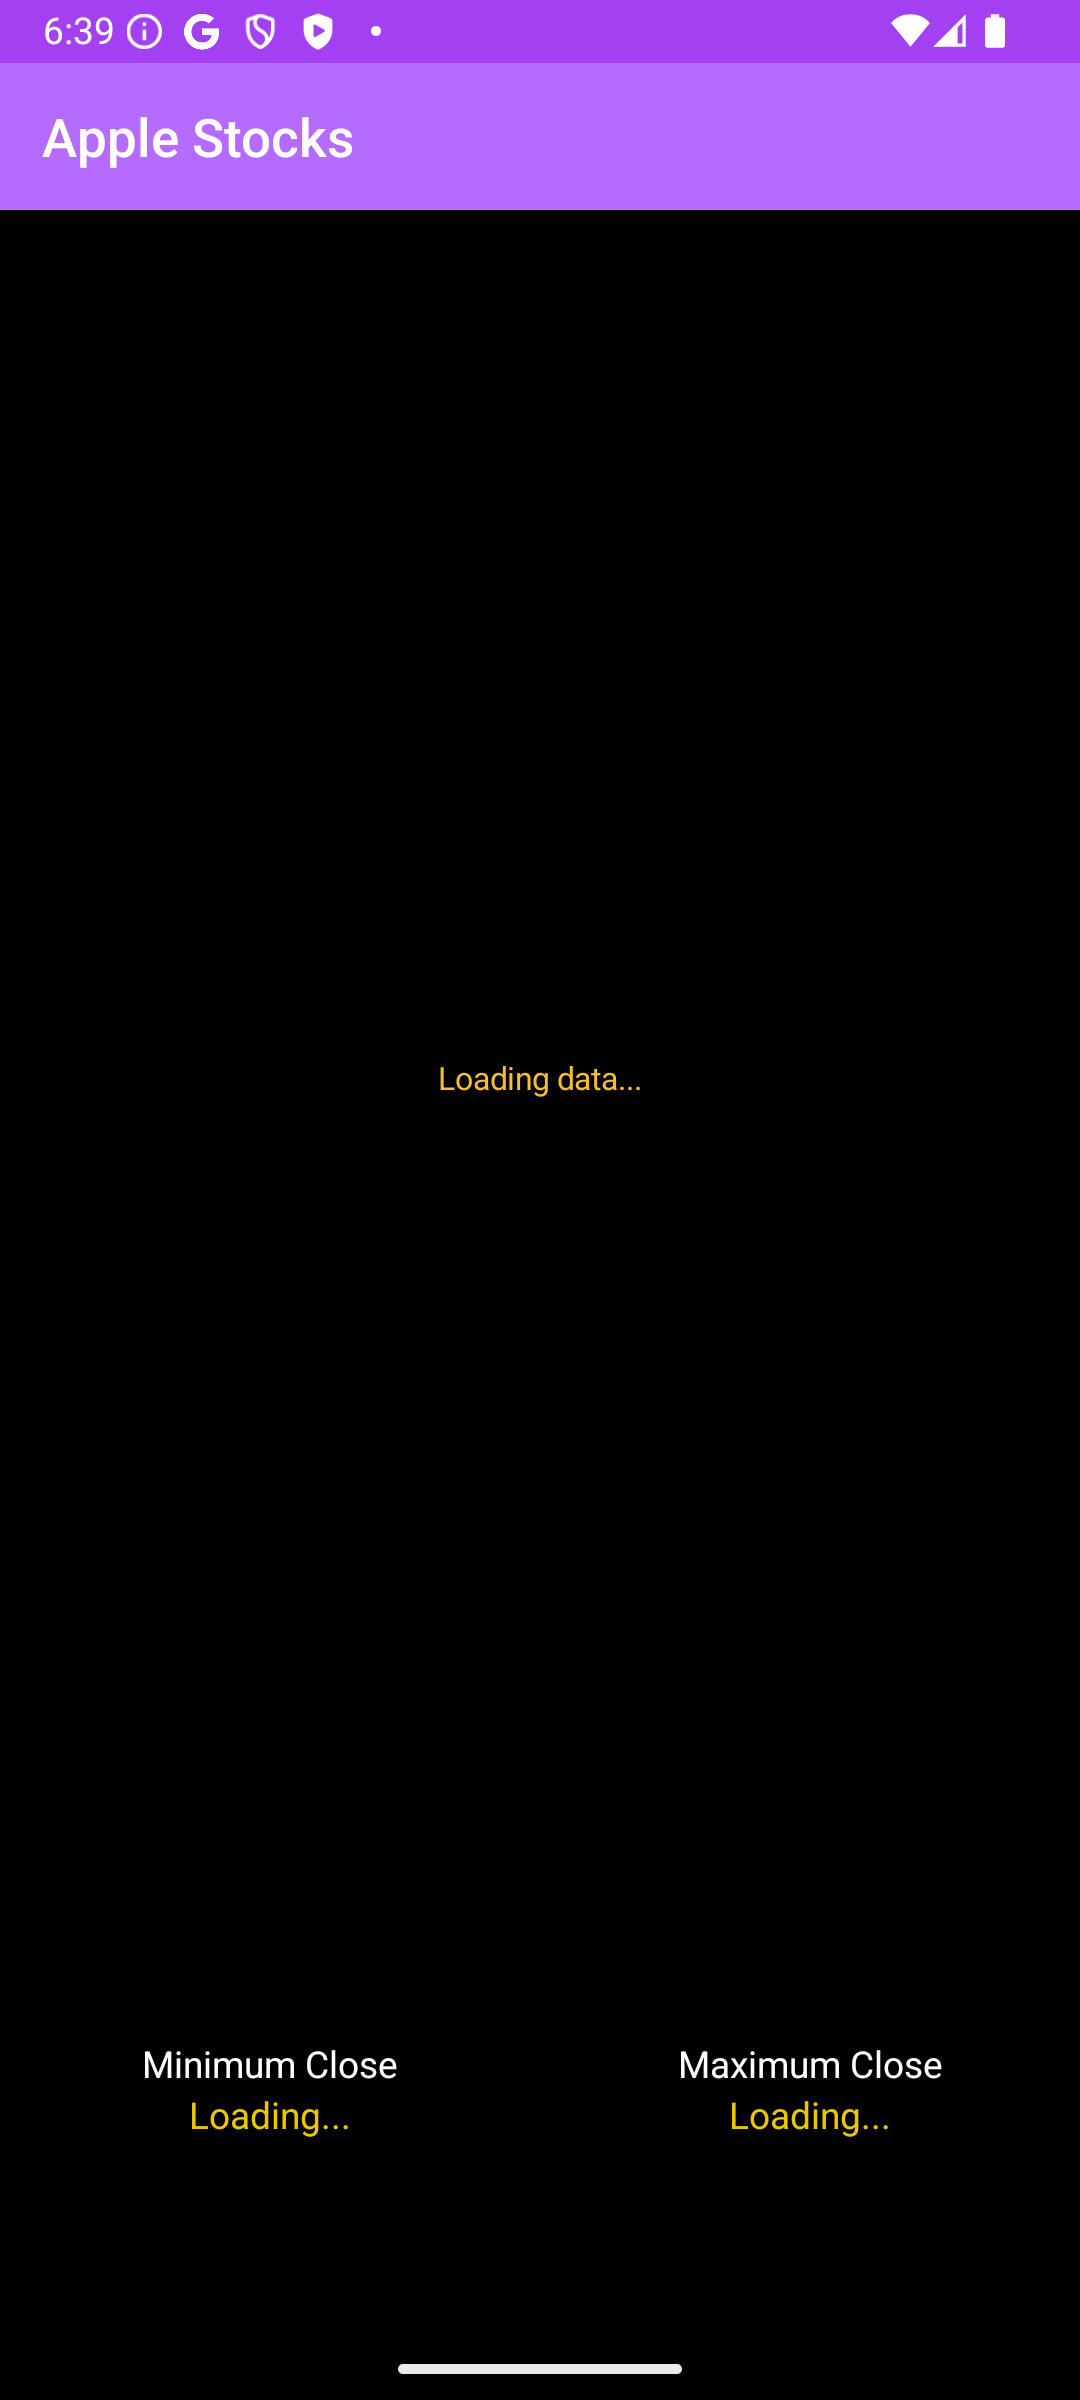
\includegraphics[height=40em]{Imagens/Loading.png}
        \caption{While Loading.}
        \label{fig:loading}
    \end{subfigure}
    \hfill
    \begin{subfigure}[t]{0.49\textwidth}
        \centering
        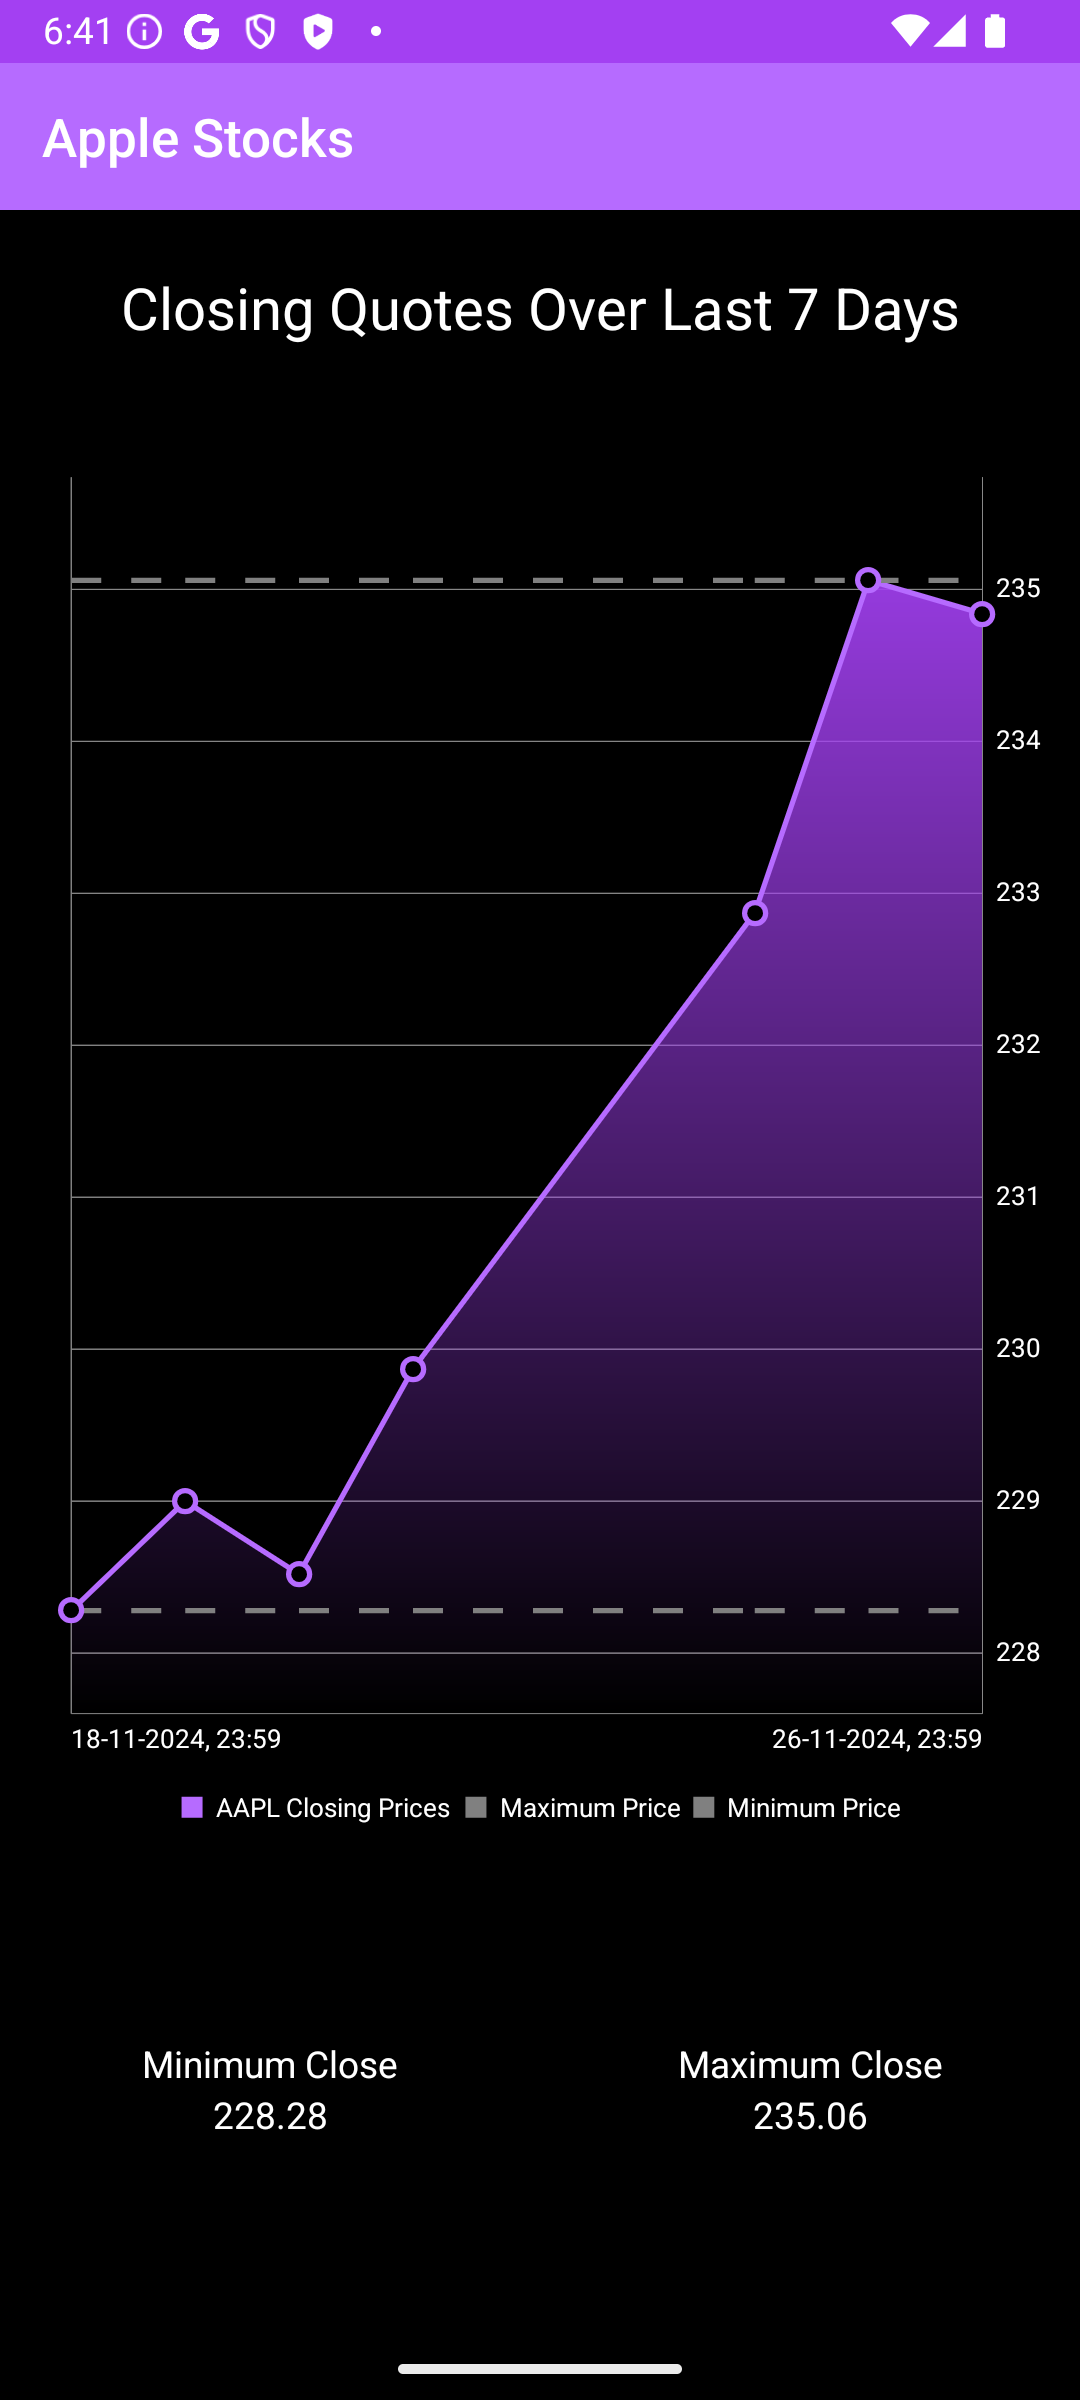
\includegraphics[height=40em]{Imagens/7days.png}
        \caption{Example for 7 Days.}
        \label{fig:plot loaded}
    \end{subfigure}

    \caption{Plot Activity.}
    \label{fig:plot activity}
\end{figure}

To have an indication of the chosen time intervals, the number of time intervals and time interval type are written in the plot title.

\subsubsection{Plot}
In \autoref{fig:plot loaded} it is possible to see how the data is plotted, in a simple and clean manner, using a color with a good contrast.
The plot is filled with a gradient to ease data visualization, when compared to having no fill, while not being too tiressome to the eyes, as a solid colorful fill would be.
As mentioned, to avoid an excess of information, only the first and last x-axis labels are written, with the title already providing enough information for the correct understanding of the graph.

Below the plot, the maximum and minimum close values can be seen, ensuring an exact reading, when compared to a reading done from the plot.
It is also possible to note the previoulsy mentioned maximum and minimum bars, in a grey dashed line, that help visualizing the results in a more graphical manner.

\subsubsection{Loading Messages}
\label{sec:loading messages}
Due to the noticed delay, and in hopes of giving some feedback to the user, the loading messages were added, acting as placeholders for the plot and \textit{extrema} values.
The color choosen was yellow, as it is costumary to exemplify warning and loading messages, and the three dots also help to signify the loading process is temporary, making the app more responsive.

\subsubsection{Landscape}
Just as in the main activity, a landscape layout was also designed, altough being very similar to the portrait layout.
This similarity, however, is intentional, as the activity has the same function, and so it should not change significantly.
The only differences are the placement of the maximum and minimum close values, that are now beside the plot, to ensure a more compact view of the plot, when compared to having the values bellow the plot.

\begin{figure}[ht]
    \centering
    \begin{subfigure}[t]{0.8\textwidth}
        \centering
        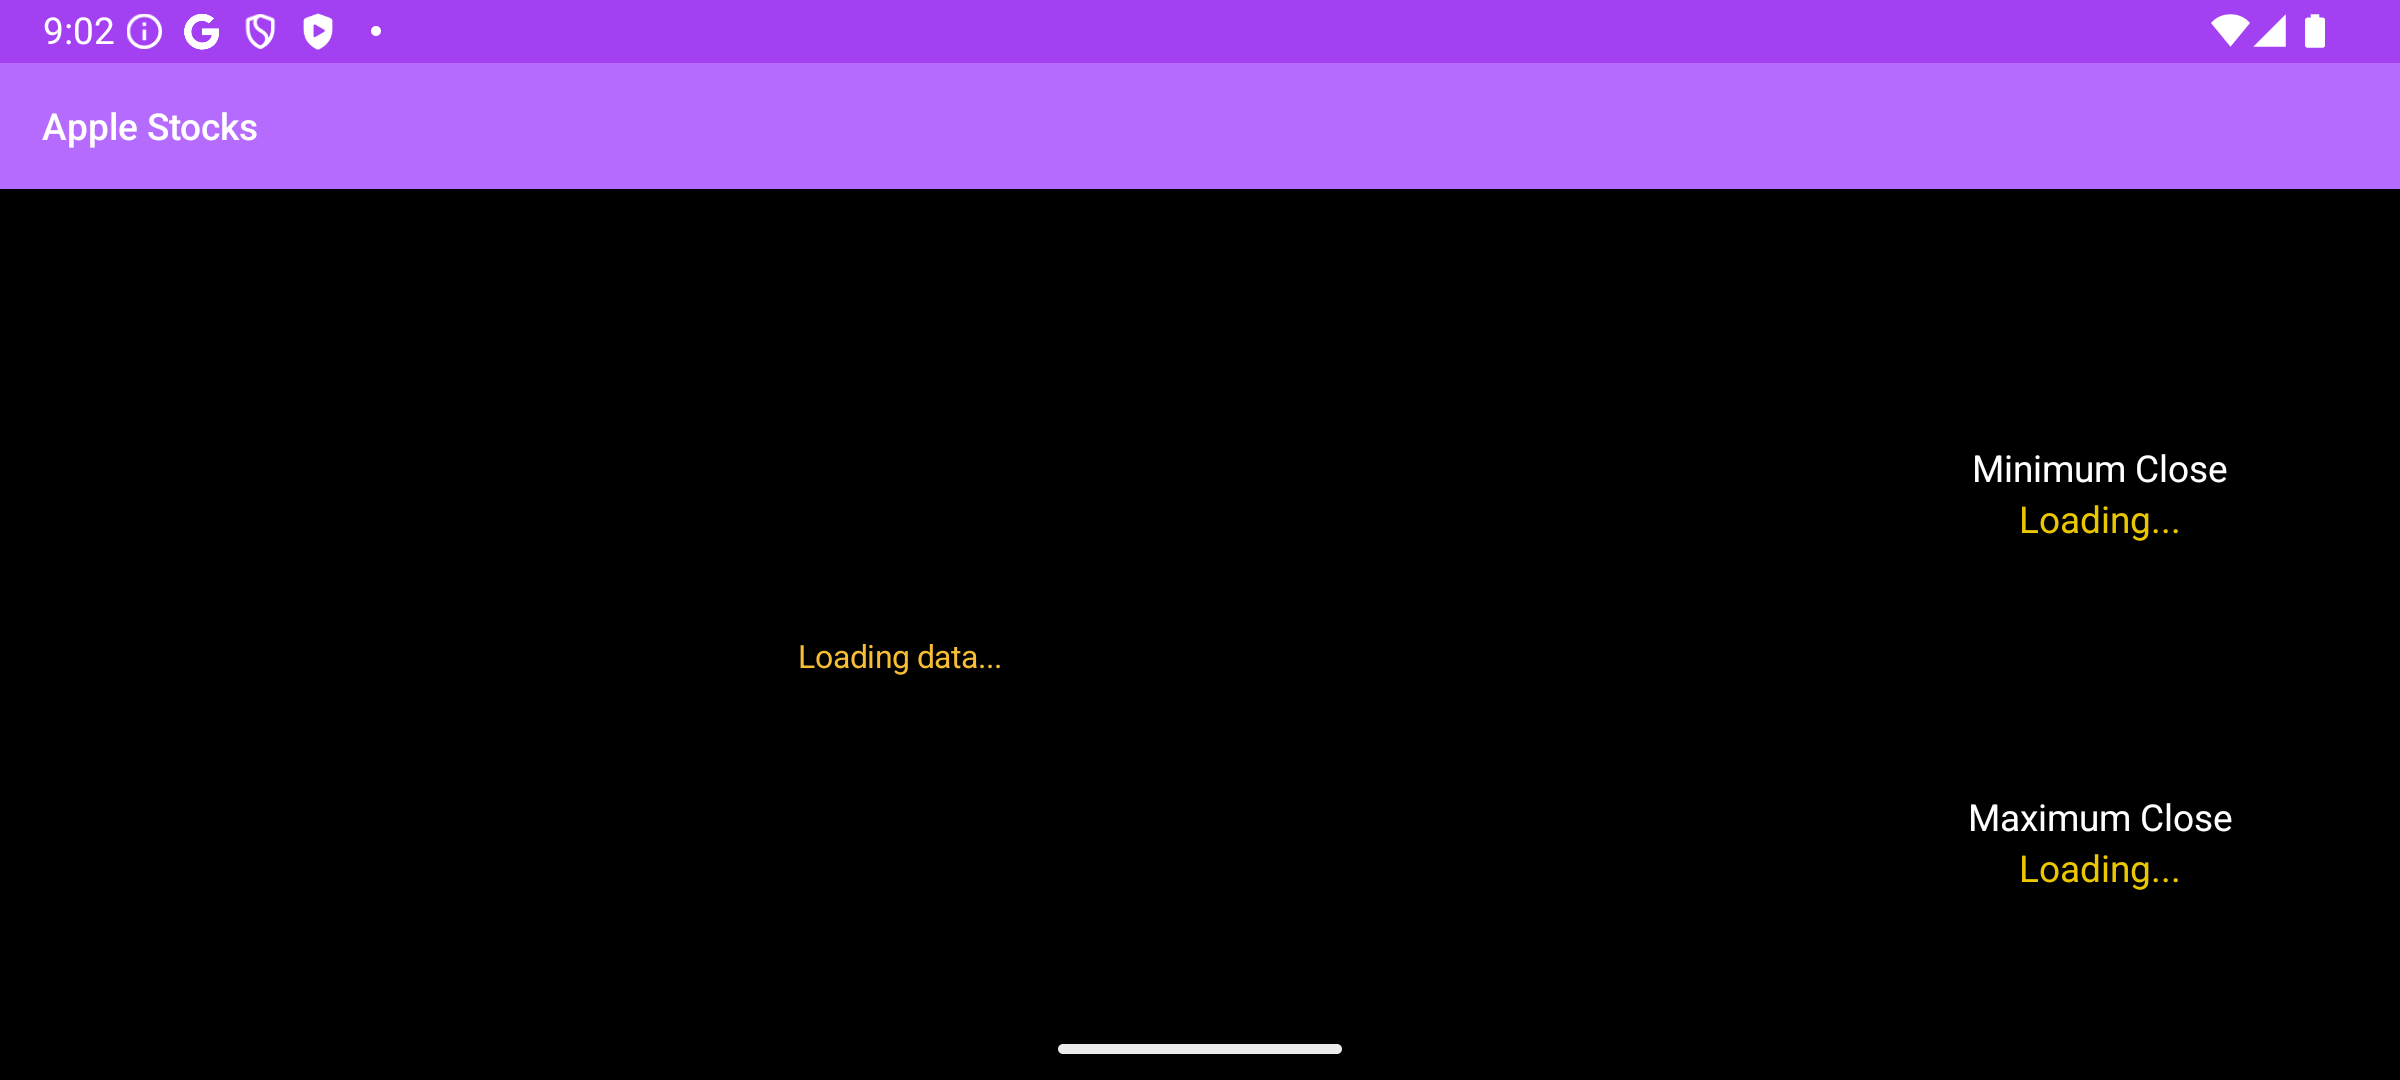
\includegraphics[width=\textwidth]{Imagens/Plot Land Loading.png}
        \caption{While Loading.}
        \label{fig:plot land loading}
    \end{subfigure}
    
    \vspace{1em} 

    \begin{subfigure}[t]{0.8\textwidth} 
        \centering
        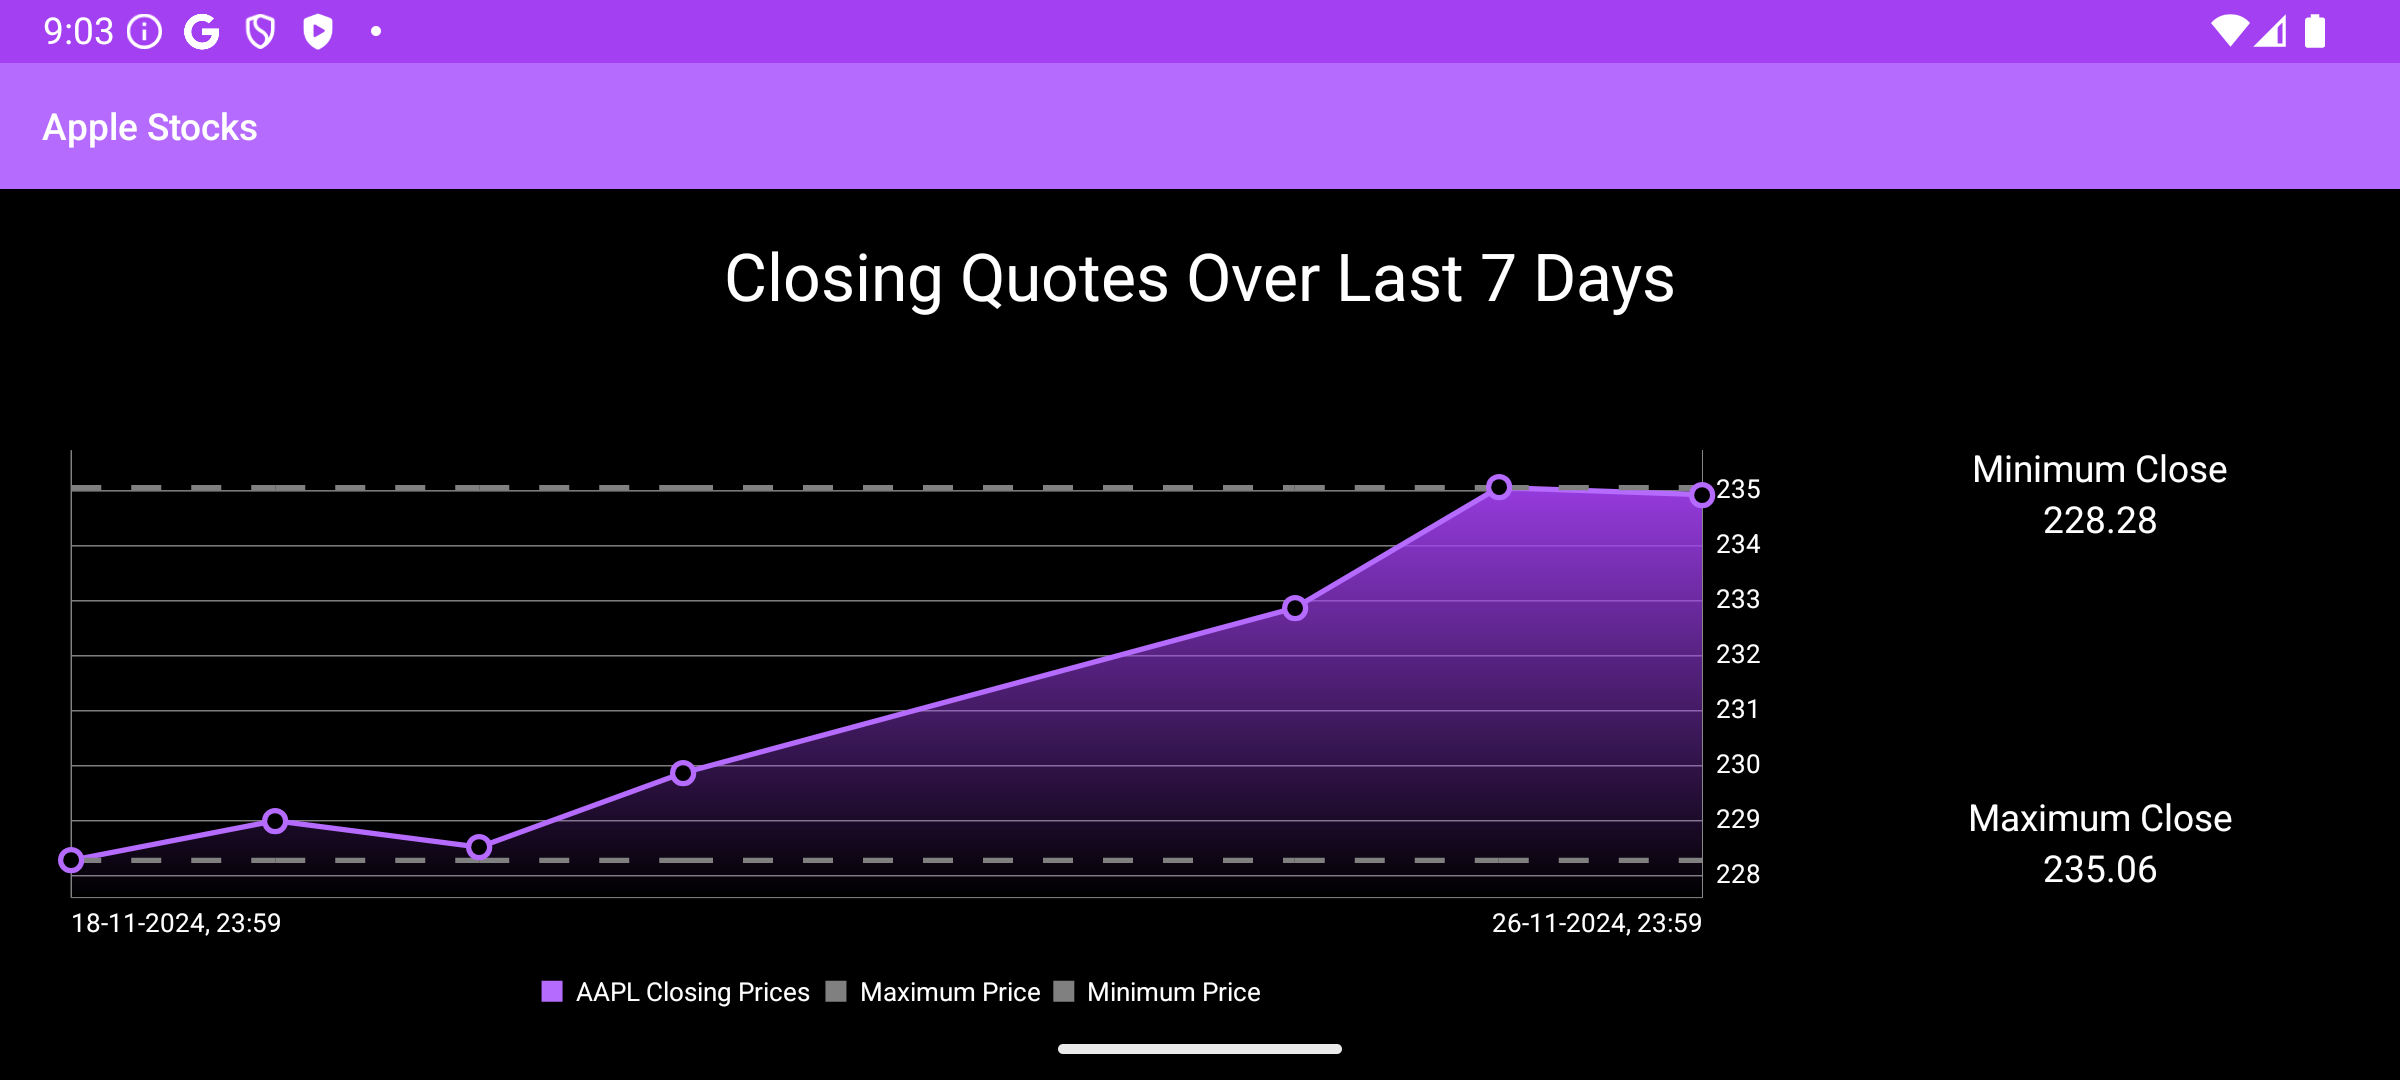
\includegraphics[width=\textwidth]{Imagens/Plot Land 7days.png}
        \caption{Example for 7 Days.}
        \label{fig:plot land 7 days}
    \end{subfigure}

    \caption{Plot Activity in Landscape.}
    \label{fig:plot land}
\end{figure}

\section{User Experience}
When presenting the interface, some key points for the user experience were already discussed, but the following aspects can be noted.

\subsection{Ease of Use}
The app provides a straightforward interface with clear instructions for users to configure their preferences.
For example, default values in the spinners (e.g., “H” for hours and “2” for the range) simplify the experience for first-time users, allowing quick access to stock quotes without additional configurations.
And the choice of spinners also helps the user to have a clear understanding of the choice they are making in regard to the time period and duration.

The layout is simple and intuitive, with the use of clear text labels and structured layouts, which also helps users less familiarized with mobile device use.

\subsection{Responsiveness}
To address potential delays caused by the API’s response time, the app includes loading messages that inform users about the current state (e.g., “Loading…”), as discussed in \autoref{sec:loading messages}. 
This feature reduces frustration and assures users that the app is actively working.

In addition, by implementing error messages, the app provides informative feedback to users, maintaining transparency and trust.
    

\subsection{Accessability}
High-contrast color themes (black background with purple and gradient accents) are utilized to ensure the interface is visually distinct and easy to read, especially in the context of financial data visualization.

The app employs a clean and minimalistic design for its data plots, avoiding overcrowding by displaying only key points on the x-axis and supplementing graphical information with textual maximum and minimum values.
Also, gradient fills enhance readability without causing visual fatigue, and dashed lines for extrema provide a quick graphical reference.

Another aspect, relevant for accessability is the landscape display, which imporves usability across various devices, including different phones and also tablets.
The landscape mode can also be seen as a source of responsiveness, as the app adjusts dinamically with the device orientation.

Finally, the app uses a darker theme, which is consistent with similar apps available on the market, aligning user expectations with the industry's visual identity.

\bibliographystyle{plain}
\bibliography{references}

\end{document}
